\documentclass[tikz,border=5mm]{standalone}
\usetikzlibrary{decorations.markings}

\begin{document}
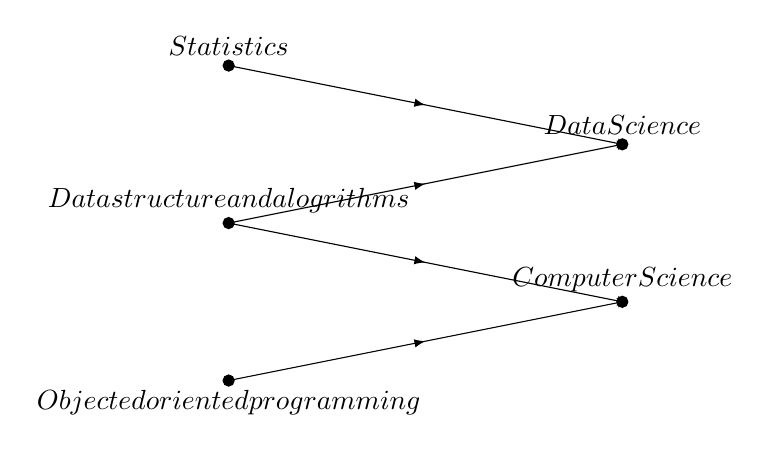
\begin{tikzpicture}
    \tikzset{
        myarrow/.style={
            postaction={
                decorate,
                decoration={
                    markings,
                    mark=at position #1 with {\arrow{latex}},
                },
            },
        },
    }

    % Vertices
    \draw[fill=black] (5,5) circle (2pt) node[above] {$Statistics$};
    \draw[fill=black] (5,3) circle (2pt) node[above] {$Data structure and alogrithms$};
    \draw[fill=black] (5,1) circle (2pt) node[below] {$Objected oriented programming$};
    \draw[fill=black] (10,4) circle (2pt) node[above] {$Data Science$};
    \draw[fill=black] (10,2) circle (2pt) node[above] {$Computer Science$};

    % Arcs
    \draw[->, myarrow=.5] (5,5) -- (10,4);
    \draw[->, myarrow=.5] (5,3) -- (10,4);
    \draw[->, myarrow=.5] (5,3) -- (10,2);
    \draw[->, myarrow=.5] (5,1) -- (10,2);

\end{tikzpicture}
\end{document}
